%%%%%%%%%%%%%%%%%%%%%%%%%%%%%%%%%%%%%%%%%
% Wenneker Article
% LaTeX Template
% Version 2.0 (28/2/17)
%
% This template was downloaded from:
% http://www.LaTeXTemplates.com
%
% Authors:
% Vel (vel@LaTeXTemplates.com)
% Frits Wenneker
%
% License:
% CC BY-NC-SA 3.0 (http://creativecommons.org/licenses/by-nc-sa/3.0/)
%
%%%%%%%%%%%%%%%%%%%%%%%%%%%%%%%%%%%%%%%%%

%----------------------------------------------------------------------------------------
%	PACKAGES AND OTHER DOCUMENT CONFIGURATIONS
%----------------------------------------------------------------------------------------

\documentclass[10pt, a4paper, twocolumn]{article} % 10pt font size (11 and 12 also possible), A4 paper (letterpaper for US letter) and two column layout (remove for one column)

%%%%%%%%%%%%%%%%%%%%%%%%%%%%%%%%%%%%%%%%%
% Wenneker Article
% Structure Specification File
% Version 1.0 (28/2/17)
%
% This file originates from:
% http://www.LaTeXTemplates.com
%
% Authors:
% Frits Wenneker
% Vel (vel@LaTeXTemplates.com)
%
% License:
% CC BY-NC-SA 3.0 (http://creativecommons.org/licenses/by-nc-sa/3.0/)
%
%%%%%%%%%%%%%%%%%%%%%%%%%%%%%%%%%%%%%%%%%

%----------------------------------------------------------------------------------------
%	PACKAGES AND OTHER DOCUMENT CONFIGURATIONS
%----------------------------------------------------------------------------------------

\usepackage[english]{babel} % English language hyphenation

\usepackage{microtype} % Better typography

\usepackage{amsmath,amsfonts,amsthm} % Math packages for equations

\usepackage[svgnames]{xcolor} % Enabling colors by their 'svgnames'

\usepackage[hang, small, labelfont=bf, up, textfont=it]{caption} % Custom captions under/above tables and figures

\usepackage{booktabs} % Horizontal rules in tables

\usepackage{lastpage} % Used to determine the number of pages in the document (for "Page X of Total")

\usepackage{graphicx} % Required for adding images

\usepackage{enumitem} % Required for customising lists
\setlist{noitemsep} % Remove spacing between bullet/numbered list elements

\usepackage{sectsty} % Enables custom section titles
\allsectionsfont{\usefont{OT1}{phv}{b}{n}} % Change the font of all section commands (Helvetica)

%----------------------------------------------------------------------------------------
%	MARGINS AND SPACING
%----------------------------------------------------------------------------------------

\usepackage{geometry} % Required for adjusting page dimensions

\geometry{
	top=1cm, % Top margin
	bottom=1.5cm, % Bottom margin
	left=2cm, % Left margin
	right=2cm, % Right margin
	includehead, % Include space for a header
	includefoot, % Include space for a footer
	%showframe, % Uncomment to show how the type block is set on the page
}

\setlength{\columnsep}{7mm} % Column separation width

%----------------------------------------------------------------------------------------
%	FONTS
%----------------------------------------------------------------------------------------

\usepackage[T1]{fontenc} % Output font encoding for international characters
\usepackage[utf8]{inputenc} % Required for inputting international characters

\usepackage{XCharter} % Use the XCharter font

%----------------------------------------------------------------------------------------
%	HEADERS AND FOOTERS
%----------------------------------------------------------------------------------------

\usepackage{fancyhdr} % Needed to define custom headers/footers
\pagestyle{fancy} % Enables the custom headers/footers

\renewcommand{\headrulewidth}{0.0pt} % No header rule
\renewcommand{\footrulewidth}{0.4pt} % Thin footer rule

\renewcommand{\sectionmark}[1]{\markboth{#1}{}} % Removes the section number from the header when \leftmark is used

%\nouppercase\leftmark % Add this to one of the lines below if you want a section title in the header/footer

% Headers
\lhead{} % Left header
\chead{\textit{\thetitle}} % Center header - currently printing the article title
\rhead{} % Right header

% Footers
\lfoot{} % Left footer
\cfoot{} % Center footer
\rfoot{\footnotesize Page \thepage\ of \pageref{LastPage}} % Right footer, "Page 1 of 2"

\fancypagestyle{firstpage}{ % Page style for the first page with the title
	\fancyhf{}
	\renewcommand{\footrulewidth}{0pt} % Suppress footer rule
}

%----------------------------------------------------------------------------------------
%	TITLE SECTION
%----------------------------------------------------------------------------------------

\newcommand{\authorstyle}[1]{{\large\usefont{OT1}{phv}{b}{n}\color{DarkRed}#1}} % Authors style (Helvetica)

\newcommand{\institution}[1]{{\footnotesize\usefont{OT1}{phv}{m}{sl}\color{Black}#1}} % Institutions style (Helvetica)

\usepackage{titling} % Allows custom title configuration

\newcommand{\HorRule}{\color{DarkGoldenrod}\rule{\linewidth}{1pt}} % Defines the gold horizontal rule around the title

\pretitle{
	\vspace{-30pt} % Move the entire title section up
	\HorRule\vspace{10pt} % Horizontal rule before the title
	\fontsize{32}{36}\usefont{OT1}{phv}{b}{n}\selectfont % Helvetica
	\color{DarkRed} % Text colour for the title and author(s)
}

\posttitle{\par\vskip 15pt} % Whitespace under the title

\preauthor{} % Anything that will appear before \author is printed

\postauthor{ % Anything that will appear after \author is printed
	\vspace{10pt} % Space before the rule
	\par\HorRule % Horizontal rule after the title
	\vspace{20pt} % Space after the title section
}

%----------------------------------------------------------------------------------------
%	ABSTRACT
%----------------------------------------------------------------------------------------

\usepackage{lettrine} % Package to accentuate the first letter of the text (lettrine)
\usepackage{fix-cm}	% Fixes the height of the lettrine

\newcommand{\initial}[1]{ % Defines the command and style for the lettrine
	\lettrine[lines=3,findent=4pt,nindent=0pt]{% Lettrine takes up 3 lines, the text to the right of it is indented 4pt and further indenting of lines 2+ is stopped
		\color{DarkGoldenrod}% Lettrine colour
		{#1}% The letter
	}{}%
}

\usepackage{xstring} % Required for string manipulation

\newcommand{\lettrineabstract}[1]{
	\StrLeft{#1}{1}[\firstletter] % Capture the first letter of the abstract for the lettrine
	\initial{\firstletter}\textbf{\StrGobbleLeft{#1}{1}} % Print the abstract with the first letter as a lettrine and the rest in bold
}

%----------------------------------------------------------------------------------------
%	BIBLIOGRAPHY
%----------------------------------------------------------------------------------------

\usepackage[backend=bibtex,style=authoryear,natbib=true]{biblatex} % Use the bibtex backend with the authoryear citation style (which resembles APA)

\addbibresource{example.bib} % The filename of the bibliography

\usepackage[autostyle=true]{csquotes} % Required to generate language-dependent quotes in the bibliography
 % Specifies the document structure and loads requires packages

%----------------------------------------------------------------------------------------
%	ARTICLE INFORMATION
%----------------------------------------------------------------------------------------

\title{Who Am I ?} % The article title

\author{
	\authorstyle{Jay Lohokare, Revati Damle and Nittin Aggarwal} % Authors
	\newline\newline % Space before institutions
	\institution{Stony brook University, New York}\\ % Institution 1
}

% Example of a one line author/institution relationship
%\author{\newauthor{John Marston} \newinstitution{Universidad Nacional Autónoma de México, Mexico City, Mexico}}

\date{December 10, 2018} % Add a date here if you would like one to appear underneath the title block, use \today for the current date, leave empty for no date

%----------------------------------------------------------------------------------------

\begin{document}

\maketitle % Print the title

\thispagestyle{firstpage} % Apply the page style for the first page (no headers and footers)

%----------------------------------------------------------------------------------------
%	ABSTRACT
%----------------------------------------------------------------------------------------

\lettrineabstract{The awareness about privacy and internet anonymity is increasing day by day given the aggressive data mining techniques used by internet service providers to capture user data. This data captured is an asset for internet companies – profiling users helps companies target adverts, and even lets them sell this data to other companies. There are many ways to achieve data privacy on the internet, which mainly deal with privacy by preventing internet companies from collecting data. Such approaches though ensure privacy, complete anonymity is sometimes unwanted. Many companies need users to be signed in to access certain features. In this paper, we present a study of various ways to achieve internet anonymity. We present internet anonymity primarily in terms of 3 aspects – IP masking, Cookie masking, Query masking. We then introduce a framework that allows users to use search engines without letting the search engine profile them. The primary purpose of this framework is to achieve anonymity by ensuring plausible deniability of data, i.e., by confusing the search engine about the identity of the user. The framework successfully prevents user profiling by using a combination of data masking techniques. We provide detailed technical details and infrastructure requirements for implementing the framework. Finally, we present a performance analysis of the framework to show that it hardly hinders user experience of using search engines. }

%----------------------------------------------------------------------------------------
%	ARTICLE CONTENTS
%----------------------------------------------------------------------------------------

\section{Introduction}
The Internet is ubiquitous today, with more than half of the world’s population having easy access to some form of internet-connected machines[10]. Internet traffic today is dominated by freemium services, which let users access most of the features for free. The free features come at the cost of targeted advertisements. Internet companies capture user data at various stages of interaction with users. The users willingly or unwillingly give a lot of data to such companies when they use all the free services on the internet. This data contains rich information about the users – preferences, educational/economic/cultural/location background, etc. Search engines are using various methods to capture data from users, to generate data profiles of users. Browsing history, location history, shopping cart, SMS, emails, call logs are call captured by these internet giants for targeted advertisements. Most of the times, users are unaware that internet companies capture their data – users usually blindly accept privacy policies and conditions without reading them thoroughly. These documents often have data capture policies hidden somewhere in them, but not many users care to read them. \newline
We conducted a study with 50 internet users to check their awareness about data capture policies of internet companies. Amongst these 90 participants - 30 were university students (From various fields of study) and the remaining 60 were people from various age groups and professions. We tried to achieve a uniform distribution of people from various professions. The study involved asking questions related to data policies of Facebook and Google. We asked a set of questions to participants to check their knowledge about what data is being captured by these companies. All our participants used Facebook, Amazon and Google services on both – PC and Mobile platforms. 	\newline
The first set of questions were of the format ‘Does X company capture Y data,’ with X being Google, Amazon, and Facebook, Y is a set of data points – Browsing history, location, SMS, email, call logs, phone usage history, shopping carts content, shopping history, location history. The 2\textsuperscript{nd} set of questions were related to internet usage behavior –
\begin{enumerate}
\item Do you read the terms and conditions, privacy policies and data policies when you signup to internet services?
\item Do you mind internet companies capturing your personal data mentioned earlier?
\item Do you use ad-blockers?
\item 	Are you willing to share your data to get improved services and recommendations?
\item 	Are you willing to share your data to get access to premium services?
\item 	Do you expect internet companies to keep your data to themselves?
\item 	Do you take any special measures to ensure internet anonymity?
\item 	Does incognito mode hide your online identity?
\end{enumerate}

The results of this study were interesting – only 38\% of participants were aware of internet companies capturing such vast amounts of data. 53\% of users were aware that companies capture data, but they were not aware of all data points used as a source of this data. Surprisingly, 81\% participants accepted to not reading the onboarding documents (terms and conditions, privacy policy). 42\% of participants users used some form of ad-blockers, while just 13\% of users took additional measures for ensuring internet anonymity. One observation was that 73\% of the users who were unaware of data being captured were not comfortable with sharing all their personal data even for premium services or improved performance. There was a near unanimous (92\%) opinion that internet companies should protect all the data they capture, and not sell it to other companies. An alarming observation was that 95\% of participants believed that incognito mode completely hid their identity online!\newline

Not only is confidential personal information a part of the data collected by such websites, but due to the rise of hacks and attacks on servers of such internet websites, this data collected is at risk of being exposed to the public. The data profiles created by internet companies from search queries often tells details about a user’s work, personal and social life. For example, searching for a costly restaurant indicates high social status. Search engines can target advertisements of similar hotels to the user. More importantly, the search engine now knows the social status and buying power of the user. The so-called incognito mode of browsers is hardly of any use. The internet companies already have mapped IP addresses with users and can easily know that the user is trying to connect without having access to the cookies.

\section{Related Project Work}
Query-based web search is an integral part of many peoples daily activities. But this search process is used to identify the individuals by the internet giants. Government requests for such logs increases the concern. To address this problem, [8] proposes a client-centered approach of plausibly deniable search. The concept of Plausible deniability is a very old one - Its ability of people to deny certain events due to lack of evidence confirming their participation. We base our study on this concept - to build a tool that ensures privacy by ensuring plausible deniability for users. This plausible deniability is achieved by IP masking, Query masking and cookie masking. As the paper suggests, just anonymizing users is less effective, as the query itself contained identifying information. The paper address this concern by generating a set of cover queries for each real query. This eliminates timing based attacks to discover the real query. While not completely hiding the real query, if done properly it supports a notion of plausible deniability. While it is possible that an individual may have issued the actual query, it is equally plausible that they issued one of the generated cover queries. This places a burden of proof on the user of the query log when trying to imply something about an individuals interests. The process of masking the user queries is what we want to emphasize on in this paper. There has been some work done in past to achieve such masking. However with dawn of deep learning, the extent to which we can achieve this masking has highly increased. We use the concept of Plausibly deniable Query set, as introduced in [8], which is a set of queries similar to the user queries that can be used to mask the users identity, but get similar results. We construct a new query from the input query using a deep learning model (LSTM). Unlike previous studies, we leverage the growing computing abilities for browsers and the increased internet bandwidth to achieve a better query set. We also include a notion of background random queries (A set of random queries run in background to confuse the advertisement targeting algorithms), and analyze efficiency of such an approach. By achieving a multiple countries based VPN, we also evaluate use of such rotating IP approach for queries.\newline
Google announced in 2007 that it will anonymize server logs that it collects every 18-24 months to protect the privacy of it users. Prior to this, google retained server log data in its original form indefinitely, which made it possible for anyone with access to those logs such as government agencies possibly gaining them through legal processes to potentially track queries back to users. Amongst the information that was stored was IP address and cookie that can help the onlooker to reach the user even if his connection changes. But this project does not anonymize the query on the fly allowing Google itself to draw conclusions on profiling the end user. That year AOL also released some anonymous data where a woman was identified based on cookie data from the captured logs. Google as of 2007 did not find a way to anonymize cookies. The Search history stored at ones computer and ISP might again reveal the identity of the user and become target for Ads. So, a solution starting from ones browser is essential. Although there are arguments against anonymization but they also forebear the need for privacy of users. The paper commands that there can be potential loss of data and data ownership [1].\newline
[2] provides two solutions to the problem of web search anonymization. One is using a client side software to inject noise queries and second is using a network of relay servers to hide the source. Our solution is inspired to take into account both the techniques by means of using a VPN server to make the queries anonymous and also by generating canonically similar queries as original ones without giving away any identity information that can be derived even after removing the IP information and cookie information. These 2 constraints are not covered by [2]. The objective of machine learning is to extract useful information from data, while privacy is preserved by concealing information. Thus it seems hard to reconcile these competing interests. [3] follows from AOL revelations and provide mechanisms by which we can not deduce the users from the search query logs too. This paper suggests the use of differential privacy to anonymize a query log. Differential privacy is the state-of-the-art approach which provides a strong privacy notion. Differential privacy provides guarantees that every individual user in the datasets would not be identified. Unlike k-anonymity, differential privacy does not make assumptions about the amount and scope of an adversaries background knowledge. The first mechanism is that the queries can be encrypted using a hash that can be decrypted if one has sufficient number of instances of that query from multiple users. The second mechanism is that the users can be divided into multiple sessions to disassociate the users from themselves. Both these methods again neglect the fact that there might be other levels where the search anonymity might be compromised.\newline
[4] provides an interesting way by which we can test whether personalized search can be done even after anonymization of user profiles is done. Usage of VPN to promote anonymity in addition to query obfuscating might not work as proposed by various organizations as Nortel as it might limit the user to certain sites as many sites these days can detect a user being operating behind a VPN and they prevent or block this access and consider it as default on IP restrictions.[5] tells us how the web search engines build user profiles to provide personalized search results to the end user based on persons past search keywords which breaches users privacy.[6] and [7] both discuss about ways in which the search engines as well as government agencies or adversaries who can lay their hands on the search query logs can trace back to users and target them appropriately. All these efforts are directed in order to identify the information that the users are revealing in hands of adversaries by means of their search queries which tend to reveal more than they should. These efforts propel for solutions on the client side to hide away the information such as IP address, gender revealing keywords, age oriented keywords etc.\newline
IP and cookies are masking are handled by many existing tools, but no tool handles query masking. With a signed in user, hiding cookie and IP prevents search engines from knowing the browsing history and location of the user. However, the Query itself contains a lot of data about the user! Let’s consider a query “Indian restaurants in Manhattan” tells the search engine that the user is interested in Indian food and is in Manhattan! Masking queries on search engines (Or similar content on other internet services) is hence essential. To summarize, internet anonymity is essentially about 3 aspects – IP masking, Cookie masking, and Query masking. \newline
While implementing the framework, we evaluated various methods to achieve each of these masking -
\subsection{IP Masking}
The IP masking is a series of techniques that are employed to hide your identity on the internet scape. The identity of the end user pertains to revealing the IP address of the device that he/she is using to access the network. The IP address, in turn, can give way to also determine the geographical location that was used to access the internet network. The IP address and geographical information can be used by the web servers and content providers to target Ads pertaining to that location such as restaurants, activities, rental properties, etc. nearby to that place.\newline 

The IP is required to be masked at all times whenever the user is trying to access the content on the web such as downloading, uploading, browsing or communicating. This varied kind of services is provided by various content providers who tend to track the activities of its users by monitoring them based on their IP addresses, their device IDs and their geographical regions. In some cases, the content providers also lay special policies for content access based on IP addresses although there might be more complicated policing practices nevertheless, the IP address tracking and monitoring is a very common and basic mechanism for a content provider to monitor the content’s usage that it has to offer on its site.\newline

The two most common practices to mask ones’ IP Address are VPNs and Proxy servers. In case of proxy servers, the end user relays its service request through the proxy server which transmits the request to the actual content provider using its own “fake” IP address and renders back the content to the end user. In this manner, each and every request has to relayed through the proxy server, and the end content provider only sees the proxy server’s fake IP address. Although every approach tries to achieve the target goal of anonymity, it also has its cons. Since each request is relayed through a server theft of info can be processed by the compromise of the server itself.\newline

Another mechanism used commonly is VPNs. VPN or virtual private network has come of age in the virtualized cloud-based paradigms developing today in the ISP world. The end user connects to the VPN network, and each request is routed through the VPN network in a secure encrypted manner to the end content provider server and is then routed back through VPN network back to the end client machine. The client machine gets assigned an IP address from the VPN provider and is used for accessing all the network services through the network which provides the anonymity to the user. Since encryption is involved in transporting each request through the VPN, the browsing involves larger latency times for rendering the content.\newline

\begin{figure}
	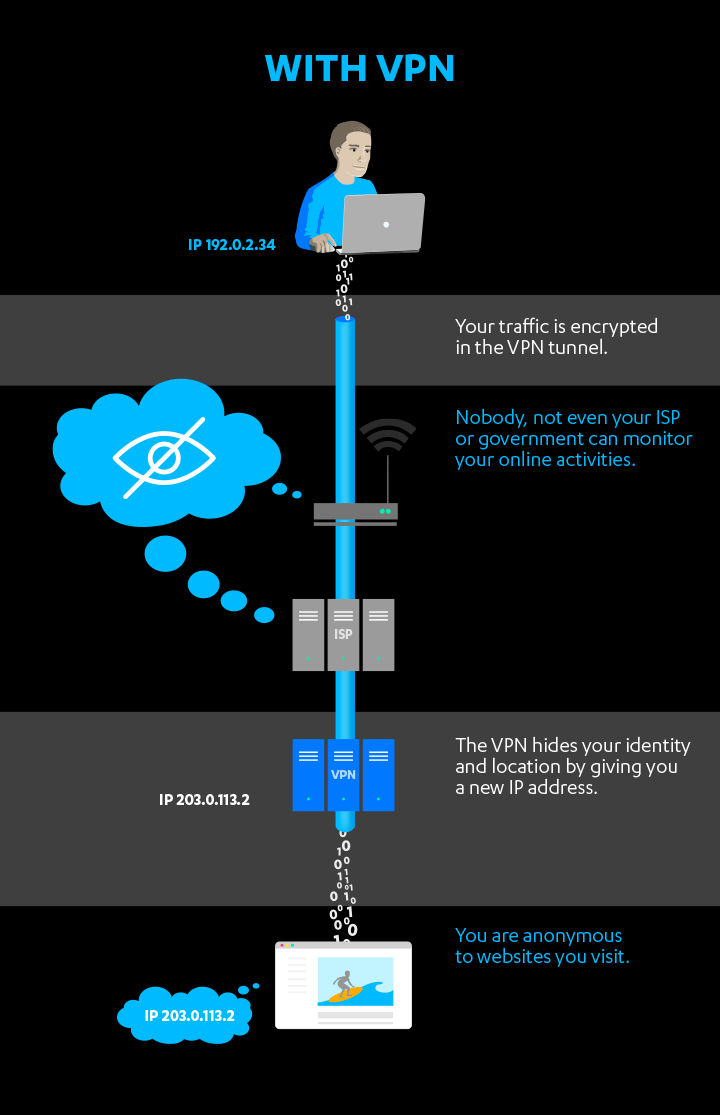
\includegraphics[width=\linewidth]{VPN.jpg} % Figure image
	\caption{Client behind VPN} % Figure caption
	\label{VPN} % Label for referencing with \ref{bear}
\end{figure}
It can be seen from the figure 1 that the client is able to connect to the VPN network through a secure encrypted tunnel which cannot be snooped by the government, ISP providers or any other external agencies. Also, it can be seen that the IP address assigned to the client is from a pool of IPs provided by the VPN provider, but the request is sourced from a different IP belonging to the VPN network.\newline

Another not so commonly used mechanism but used by the researchers and students is a TOR browser. The TOR browser is like any other browser such as Safari, IE or Chrome but it uses a set of relays across its network for processing the requests which make the processing of request anonymous but costly in terms of time.
\newline

\subsection{Cookie Masking}

There are other ways and data points which can be used to compromise the identity of the user, and these ways are even more dangerous and more intruding than the IP counterpart as it can reveal not only the identity of the user, geography of the user but the tastes, chats, searches, keywords, login activities, clicks, views to the website whose content is being browsed by the client which can help in profiling the users based on his/her tastes and designing even more specifically targeted Ads. All of this information can be extracted from the cookies which are plain text of information sent by the server rendering the content for the first time when the client lands on their site, to the client so that it can remember the site visits the next time the user lands on the same web page by looking at the cookies shared by the client this time with the server. The set cookie header in the HTTP request is a common way the websites take care of the first party cookies in the picture.\newline
Other kinds of cookies such as flash cookies and tracking cookies are also employed by the web servers by embedding them in the images, videos and other content viewed in their site by the client user. The most common misuse of the cookie information is made by the Airline reservation sites where they make use of the cookies to detect that the user has visited the site again and may intend to purchase the ticket and this prompts them to show a slightly higher prices in the site whereas they show different prices for the first time visitor to the site.\newline

There have been many ways for the informed or the concerned of the users whose demands have been answered by the browser developers who have included various configurable options for the end user to select to block the use of cookies for rendering their request for services inside the browser. There are simple options in the privacy and security section of the preferences dialog box of the various browsers such as disable the third party cookies, create TPLs or tracking protection lists, disable the Ad personalizations, etc which to some extent do not share the cookies with the end servers. There is also a private browsing mode supported by many browsers which is also termed as the incognito mode in Google Chrome which does not store the cookies persistently. There are a couple of plugins as well such as Google analytics browser add-on which does not let Google use our data for pointing Ads at us and profiling us. Ghostery helps us in evading the tracking cookies and helps in faster page loads and protects data shared by the user on the sites.\newline

In spite of all these efforts, the web servers might be able to collect data from the user by way of queries searched or browsed by the user reflecting a glimpse of themselves which might be learned by the web servers over time and can target Ads at us. The DuckDuckgo browser is recommended by the researchers these days as it claims that it does not track its users’ activities by means of cookies and IP address and gives an experience of anonymous browsing but it is not all that true to believe as it might also employ other tactics to improve the search experience of the end user and this takes us to investigate the use of the search queries made in the browser to search for the content wished by the end user.

\subsection{Query Masking}
This is the main feature that we are focusing on this re-search project. The queries made by users on web search engines like Google, Yahoo, etc. reveal sensitive details of users and their data profiles. Such information is used by the engines to create a web profile on them and recommend the users with the most irritating advertisements. In addition to this, most of the users are uncomfortable sharing such in-formation and consider it a violation of ethics. Most existing tools handle IP/Cookie masking, but no tool handles masking of search engine queries which is the need of the hour. We have explored various methods to anonymize the queries using Natural Language Processing (NLP). Primarily we classify our approach into two parts: Statistical/Machine learning approaches, and Deep Learning-Machine Translation.\newline
Machine learning approach includes the traditional Natural Language Processing (NLP) techniques. It is a two-step process where we use POS tagging and Word-to-vector to find similar words. The Part-of-speech (POS) tagging reads the text in a language and assigns parts of speech tags to each word in the query. It tags a token with noun, verb, adjective, etc. A wide variety of software and libraries are available which provide such taggers, which tag the sentences from lowest of the levels like nouns, adjectives to the complicated analysis of part of speeches like noun-plural, etc. The most widely used POS taggers come from Python’s NLTK and scaCy packages.
\begin{center}
\begin{tabular}{ |c|c|c|c|c| } 
 \hline
 A & tall & boy & ran & home \\ 
 \hline
 DT & JJ & NN & VBD & NN\\ 
 \hline
\end{tabular}
\end{center}
We can use various ways to get the complicated levels of tags that we need using the two packages. The next level of tagging many applications find useful is the Named Entity Recognition (NER) tagging. The technique consists of recognizing entities in a sentence like Person, Location, Nationalities, etc. The most widely used package for NER tagging is CoreNLP. The annotator in CoreNLP uses one or more machine learning sequence models to labels entities. It can also use rule-based components such as for labeling and recognizing time and dates. It is also alternatively called entity chunking/extraction. This technique is very popular in information extraction to identify and segment entities and to categorize them under defined categories. NER tagging is helpful in our scenario especially, as this will extract sensitive information which we can censor or change according to the entities they belong to. Once we get the required entities belonging to profiling categories like Location, Company names, Nationalities, we can use Word-to-Vector to find the most similar words to those categories and create multiple random related queries.\newline
Computers interact with humans in programming languages which are very structured. However, human language has a lot of ambiguity with multiple words which have the same semantic meaning.  There are words which are antonym in nature and words that behave differently when used as different parts of speech. There are various ways in which humans can comprehend a given sentence.To represent the world of language mathematically, we can represent each word in an N-dimensional space, and the N-dimensional vectors would represent the words in the language. The more similar the vectors are, the more semantically similar the words are.  Word-to-vector is a way to accomplish this. The traditional way of representing words is by using one-hot vector which is essentially a vector with only one target element being 1 and the others being 0. Though this representation is easy to understand there are several issues with it. There is no way to infer relationship between two words. Along with this, there would be numerous redundant “0” in the vectors which leads to a lot of space wastage.\newline
Word to vector is a two-layer neural net that processes text. Its input is a text corpus and output is a vector space, feature vector for words in the corpus. Word-to-vec turns text into a numerical form that deep nets can understand. Word-to-vec is implemented by various Python libraries like gensim, Deeplearing4j, etc. Using word-to-vector we get semantically related words to the sensitive words that we picked out from the sentence using POS and NER tagging. By replacing these words, we create random related queries. When these queries are issued along with the actual user query, the search engine gets confused and is not able to profile the user anymore based on his search preferences.\newline
The second approach is Deep Learning/ Machine Translation. This approach involves using neural network architectures for text anonymization. We studied various machine translation approaches that can be used to achieve this. We also have created various codes involving different architectures like CNN, LSTM, BLSTMs in order to achieve the machine translation. For this project update, we have not completed the implementation of the machine translation, and just have explored the various possible ways to achieve it. Machine translation is conversion of text by a computer, with no human involvement. Pioneered in the 1950s, machine translation can also be referred to as automated translation, automatic or instant translation. Machine translation is generally used to convert text from one language to another, while we want to convert from English to well, English. Luckily, such amazing work has been done in this paper. Even though Bulyko and Ostendorf [11] introduced the concept of using weighted finite state transducers to create multiple input sentences for a synthesizer, that doesn’t seem to work well in our scenario as it deals with domain specific queries and what we want is a generalized synthesizer. For the first project update we have explored thoroughly on various methods to convert from one English query to another with a similar meaning. To train an English to English machine translation system, a we would need a parallel monolingual English text corpus. As same-language machine translation corpora for synthesis are not available, we will develop a small corpus suitable for a this project. We would be using The ARCTIC [12] corpus, as a starting point for the MT corpus.\newline
The next part is to develop a machine translation technique. As suggested in the paper mention above, we would be using a SMT approach. Statistical machine translation (SMT) is a machine translation paradigm where translations are generated on the basis of statistical models whose parameters are derived from the analysis of bilingual text corpora. The concept presented in the paper is to use the N-best hypotheses from the machine translation system as input to the synthesizer, which is included in future work. \newline
The framework we implemented uses a combination of these approaches to achieve ‘plausible deniability.’ Plausible deniability is the ability of people (typically senior officials in a formal or informal chain of command) to deny knowledge of or responsibility for any damnable actions committed by others in an organizational hierarchy because of a lack of evidence that can confirm their participation, even if they were personally involved in or at least willfully ignorant of the actions [13]. The framework we implemented achieves anonymity by plausible deniability. The implementation is as follows – 

\section{Implementation}

The framework consists of 3 main components – 
\begin{enumerate}
\item Firefox plugin (User interface)
\item Flask server + Headless browser (Query masking, Cookie masking)
\item VPN network (IP masking)
\end{enumerate}
\begin{figure}
	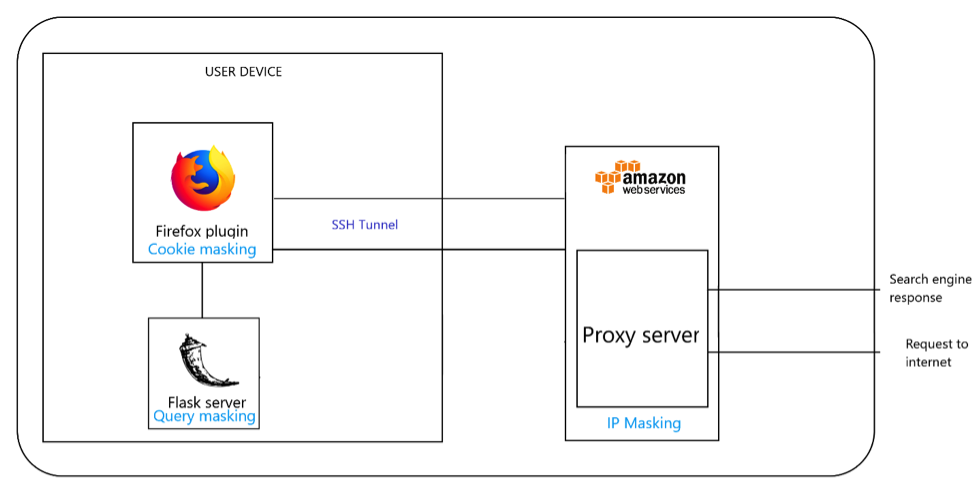
\includegraphics[width=\linewidth]{arch.png} % Figure image
	\caption{Components of System Implementation} % Figure caption
	\label{ARCH} % Label for referencing with \ref{bear}
\end{figure}
The firefox plugin is the user interface to the framework we implemented. The plugin has an interface to enter the query the user wants to search on the search engine. The firefox plugin (JS script) captures the query entered by the user and routes it to the flask server (Python). In the flask server, we have implemented a headless browser that sends requests to the search engine. To achieve cookie masking, we make requests to Google search engine via this headless browser instead of user browser and then redirect the response to the user browser. This allows removing any cookies from the requests sent to the search engine.  \newline
\textbf{IP masking using VPN network:}\newline
IP masking has been employed by utilizing the proxy server approach acting as the SOCKS5 host for our client. All the queries are entered in the search bar of the Mozilla plugin, and they are required to be routed in a way that they do not expose the IP address of the client machine. \newline
Also, it is required that the similar alternate queries that are generated by the python flask server are routed anonymously to the Google search engine page. To achieve this, a setup comprising of 6 Proxy servers running as separate instances in the Amazon EC2 cloud. The instances have been created in separate regions of the World namely Bangalore(India), Vancouver(Canada), New York(US), London(UK), Capetown(South Africa) and Sydney(Australia). These regions have been created in separate instances thus they have 6 different IP addresses which are randomly chosen to route the queries. The algorithm to choose the IP addresses currently employed is round robin, but it can be chosen by any other selection algorithms too.\newline
The query that is originally fired from the plugin generates 5 similar alternate queries, and all of them are run or routed through different EC2 instances and hence they are sourced with 6 different IP addresses. The random IP address selection plus the utilization of fake IP addresses for sourcing the queries masks the true IP address of the client and confuses the snooper about the true identity and location of the client searching the content on its search engine. Although the implementation is able to take care of the anonymity, it comes with a disadvantage as has been seen with various IP masking approaches i.e. it's not able to take care of the latency part well. There is an added latency pertaining to the time required to route through one region to another from the original region of the client.

\textbf{Query Masking}\newline
The implementation of query masking is achieved in two parts: Tagging and Word-to-vector words similarity. Tagging is achieve using spaCy, a free open-source library for NLP in Python. It features NER, POS tagging, dependency parsing, word vectors and more. It provides two levels of tagging. The first one is part of speech tagging which tags words into Nouns, Adjectives verbs etc. The next level of tagging, is Named-Entity-Recognition tagging, which categorizes words into entities like Nationalities, Locations, Time/Date etc. Consider the query, “Indian restaurants near me today in NYC”, when passed through POS tagger, gives us the following tags:
\begin{center}
\begin{tabular}{ |c|c|c|c| } 
 \hline
 Indian & Restaurants & today & NYC \\ 
 \hline
 ADJ & NN & ADV & NN \\ 
 \hline
\end{tabular}
\end{center}
The next level of tagging is Named Entity Recognition tagging which is also a part of spaCy package. As per the spaCy documentation, a named entity is a "real-world ob-ject" that's assigned a name – for example, a person, a coun-try, a product or a book title. spaCy can recognize various types of named entities in a document by asking the statisti-cal and strongly trained model for a prediction. Even though this might not give perfectly similar words, the queries that are made with this approach are random enough to confuse the web search engine. In the above example, the NER tag-ging happens as follows:
\begin{center}
\begin{tabular}{ |c|c|c|c| } 
 \hline
 Indian & Restaurants & today & NYC \\ 
 \hline
 NOPR &  & DATE & GPE \\ 
 \hline
\end{tabular}
\end{center}
Here NOPR is Nationalities, DATE is a date tag and GPE signifies countries, After extracting words that belong to these categories, that give out profiling information on the user to the web search engine, we try to find most similar words to them using word-to-vector. We have used gensim library provided by Python for this purpose. We extract the words from a query which belong to such entity categories and then use word-to-vec embeddings to replace them with the most similar ones. For the embeddings we have used gensim’s GoogleNews vectors model which contains around 3 million words that are trained on Google news dataset. Using the combination of these two techniques, we were able to general related random queries to the above query such as:\newline
\textbf{Pakistani} restaurants near me \textbf{tomorrow} in \textbf{L.A}\newline
\textbf{Italian} restaurants near me \textbf{yesterday} in \textbf{S.F.} \newline
Here we find replacements for words like “Indian”, “to-day” and “NYC” which give out profiling information to the search engine and helps it to conclude that the user like Indian food and is in NYC today. When we replace them with words like “Pakistani” or “Italian”, change the location and the time, the engine gets confused and is not able to make an inference on the user’s preferences. Thus, this helps the user to safeguard his privacy.\newline
The headless browser routes user query through the VPN, at the same time it also creates multiple relevant queries and routes them through the VPN (albeit from a different region). This essentially confuses the search engine – The search engine sees multiple cookie-less queries coming from different countries at the same time for the same user, that too with each query content being different from the other. This results in plausible deniability, as the search engine is now unable to detect which query represents the real user. The search engine now has user data, but most of it is junk data. The user’s identity remains hidden even if this data is compromised. In case the data captured by search engines is attacked and leaked, the user’s true profile can never be found as the search engine itself isn’t aware of the user’s true profile. The search engine might still target advertisements to users based on the junk data they have. These advertisements will be junk (As they won’t be related to user preferences at all). The future scope of this framework includes adding an add-blocker for blocking such junk advertisements).
\begin{figure}
	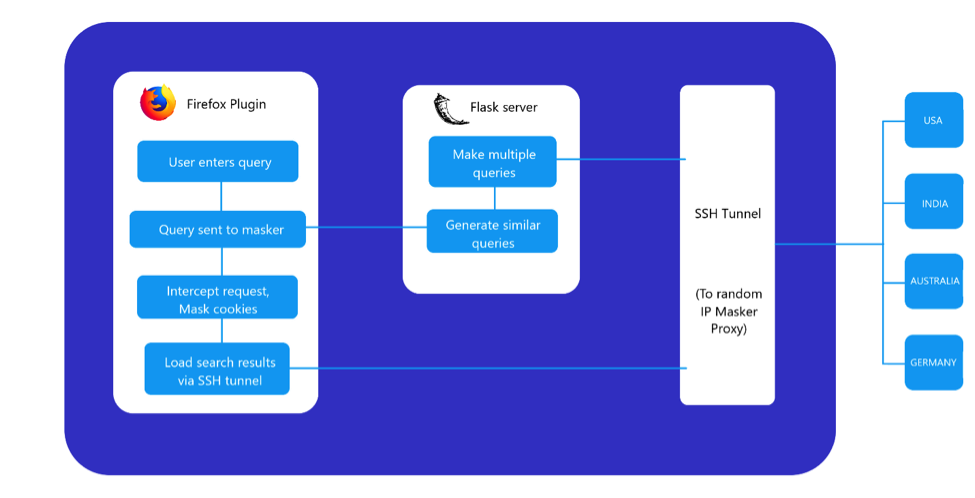
\includegraphics[width=\linewidth]{Flow.png} % Figure image
	\caption{Data Flow} % Figure caption
	\label{Flow} % Label for referencing with \ref{bear}
\end{figure}
\section{Example Use Case}
Suppose a user wants to search for a query “Indian food in Manhattan on 30\textsuperscript{th} January”. The user will first install the firefox plugin. Then, the user will enter the query in the plugin interface. The plugin will then make API call to send this query to Flask server. The flask server will create a new HTTP request to Google search engine, with the request having no cookies related to user’s browser history. The flask server will send this query to the request handler which is connected to the VPN network. At the same time, the flask server will also create 8 similar queries (Using query generator) and send them to the request handler. All these requests will contain the user session details, but no browsing history. The request handler will then randomly select a country to route the request from. The request is routed via the proxy server setup on AWS EC2 in the selected region. For the considered example, the following is an example of what could happen – \newline
Indian food in Manhattan on 30\textsuperscript{th} January – Routed through USA\newline
American food in LA on 27\textsuperscript{th} January – Routed through India\newline
Chinese food in London on 26\textsuperscript{th}December – Routed through London

\section{Performance}
We evaluated the performance of this framework to verify that user experience is not hampered. The framework ensures privacy, but it should not be at the cost of user experience. We evaluate response time, increase in computing requirements and memory requirements for this framework. In our experimental setup, we use a non-production flask server with debugging off (to minimize memory and computing resources usage). For comparing the performance, we ran a set of queries directly on Google and then did the same using our framework. The evaluation of performance was measured using Apache JMeter (For network related parameters) and shell scripts to monitor memory and CPU usage. We ran 100 queries each (With and without our framework) and noticed a 134\% increase in network response time. We associate this increase in response time to the fact that we route the requests through servers in different countries. We also evaluated the memory footprint of the Flask server that runs in the background. We tested the framework (with firefox plugin) on PCs with various configurations. The shell scripts we used to monitor memory usage of our framework showed us an average memory usage increase of 300Mb. Analysis of the system showed us that Flask server itself takes around 250-280Mb memory (Without any NLP models running). Adding the query generator and VPN router thus adds a nominal memory footprint to the system. One of the future scopes for our project is using a lightweight alternative to Flask, thereby making the framework lightweight.  \newline
The cost of implementation for our system is dependent on the cost of hosting infrastructure (Cloud) for achieving 
A VPN. The current implementation is free for 1 year (Due to EC2 free tier), but will cost 53\$ per year for hosting.

\section{Future Work}
The Future scope of this framework mainly includes ways to make the system lightweight. There are many compute heavy and CPU intensive components used in the framework. The Flask server as seen in our analysis consumes a lot of RAM and CPU, making it imperative to find a lightweight alternative. Another scope of improvement is connecting to free VPN services instead of deploying custom VPN to reduce infrastructure costs. Another aspect that can be worked on is the introduction of adblocker to the framework. This will make the system truly end to end, preventing privacy issues and also blocking advertisements. The existing frameworks work only on firefox (As we developed the firefox plugin). By developing similar plugins for other browsers, the entire system can be used for any other browser (As all other components can be used as they are). 

\section{Conclusion}
The framework presented in the paper is one of its kind as it tries to handle all the three main aspects of data privacy and checkpoints each aspect through a simple to implement the solution. It is a strong step in the debate over privacy versus personalization. Personalization comes at a greater cost of losing all privacy at the hands of third parties with whom the user does not have any interactions at all or basically it does not have any legal consent. Although there is some scope in its development for use in the scale for it needs to be pruned enough using various system engineering techniques and become lightweight so that it might be used in various mobile domains as well where the efficiency matters second to its weight in terms of resource usage.
\begin{thebibliography}{unsrt}
\bibitem{}
 Ron A. Dolin \emph{Search Query Privacy: The Problem of Anonymization}
\bibitem{}
Sai Teja Peddinti \& Nitesh Saxena \emph{Web Search Query Privacy: Evaluating Query Obfuscation and Anonymizing Networks}
\bibitem{}
Eytan Adar \emph{User 4XXXXX9: Anonymizing Query Logs}
\bibitem{}
Yun Zhu, Li Xiong \& Christopher Verdery \emph{Anonymizing User Profiles for Personalized Web Search}
\bibitem{}
Mangesh V. Bedekar, Bharat Deshpande \& Ramprasad Joshi \emph{Web Search Personalization by User Profiling}
\bibitem{}
Deepa Anand \& Bonson Sebastian Mampilli \emph{User Profiling Based on Keyword Clusters for Improved Recommendations}
\bibitem{}
Kenneth Wai-Ting Leung \&  Dik Lun Lee \emph{Deriving Concept-based User Profiles from
Search Engine Logs}
\bibitem{}
Mummoorthy Murugesan \& Chris Clifton \emph{Providing Privacy through Plausibly Deniable Search}
\bibitem{}
Sicong Zhang, Hui Yang \& Lisa Singh \emph{Anonymizing Query Logs by Differential Privacy}
\bibitem{}
https://en.wikipedia.org/wiki/\newline Global\_Internet\_usage
\bibitem{}
Bulyko \& M. Ostendorf \emph{Efficient integrated response generation from multiple targets using weighted finite state transducers,” Computer Speech and Language}(vol. 16, no. 3, pp. 533–550, 2002.)
\bibitem{}
J. Kominek \& A. Black \emph{The CMU ARCTIC speech databases for speech synthesis research,” Language Technologies Institute, Carnegie Mellon University, Pittsburgh, PA, Tech. Rep. CMULTI03-177}(http://festvox. org/cmu arctic, 2003.)
\bibitem{}
https://en.wikipedia.org/wiki/Plausible\_deniability
 
\end{thebibliography}
\end{document}
